\documentclass[english, aspectratio=169]{beamer}
% english is for the language used in standard texts (figures, tables etc)
% aspectratio of 16:9 or set it for more old school to 4:3 (without the ':')

% ---------------------------------------------------------------------------- %
% Load base preamble
% ---------------------------------------------------------------------------- %
\usepackage{import}
\subimport{../preamble/}{beamer.tex}

% ---------------------------------------------------------------------------- %
% Local settings
% ---------------------------------------------------------------------------- %
\newcommand{\B}[0]{\ensuremath{\mathbb{B}}}

\newcommand{\sort}[0]{\text{sort}}

\newcommand{\triple}[3]{\ensuremath{(#1, #2, #3)}}
\renewcommand{\arc}[3]{\ensuremath{#1 \xrightarrow{_{#2}} #3}}

\tikzstyle{plot_adiar}=[color=black, mark=o, mark size=1pt, line width=0.7pt]
\tikzstyle{plot_buddy}=[color=red, mark=o, mark size=1pt, line width=0.7pt]
\tikzstyle{plot_cudd}=[color=blue, mark=diamond, mark size=1pt, line width=0.7pt]
\tikzstyle{plot_sylvan}=[color=purple, mark=square, mark size=1pt, line width=0.7pt]

% Horizontal legends: https://tex.stackexchange.com/a/101578
% argument #1: any options
\makeatletter
\newenvironment{customlegend}[1][]{%
    \begingroup
    % inits/clears the lists (which might be populated from previous
    % axes):
    \pgfplots@init@cleared@structures
    \pgfplotsset{#1}%
}{%
    % draws the legend:
    \pgfplots@createlegend
    \endgroup
}%

% makes \addlegendimage available (typically only available within an
% axis environment):
\def\addlegendimage{\pgfplots@addlegendimage}
\makeatother

% ------------------------------------------------------------------------------
% TITLEPAGE
% ------------------------------------------------------------------------------
\title{Decision Diagrams in External Memory}

\author{\textbf{Steffan Christ S\o lvsten}}

\institute{
\includegraphics[width=0.2\linewidth]{../external/aulogo_uk_var2_black.eps}}

\date{MOVEP 2022}

\begin{document}

\titleframe

\begin{frame}[plain,noframenumbering]{} % \blankframe until reveal
  \pause

  \begin{center}
    \vspace{8pt}

    {\Huge \textbf{Adiar}}

    \vspace{12pt}

    \textcolor{gray}{\small
      \href{http://github.com/ssoelvsten/adiar}{github.com/ssoelvsten/adiar}
    }
  \end{center}
\end{frame}

\begin{frame}
  \begin{figure}
    \centering
    
    \begin{tikzpicture}
      \begin{axis}[%
        width=0.70\linewidth, height=0.42\linewidth,
        every tick label/.append style={font=\scriptsize},
        % x-axis
        xlabel={number of BDD nodes},
        xmajorgrids=true,
        xmin=51000000,
        xmax=300000000000,
        xmode = log,
        % y-axis
        ymin=10,
        ymax=1000000,
        ylabel={Time (seconds)},
        ytick distance={10},
        ymode=log,
        yminorgrids=false,
        ymajorgrids=true,
        grid style={dashed,black!20},
        ]     
        
        \only<2-> {
          \addplot+ [style=plot_cudd]
          table {./data/queens_cudd_time.tex};
        }

        \only<2-> {
          \addplot+ [style=plot_sylvan]
          table {./data/queens_sylvan_time.tex};
        }
        
        \only<3-> {
          \addplot+ [style=plot_adiar]
          table {./data/queens_adiar_time.tex};
        }
      \end{axis}
    \end{tikzpicture}

    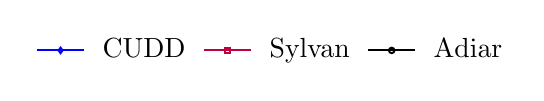
\begin{tikzpicture}
      \begin{customlegend}[
        legend columns=-1,
        legend style={draw=none,column sep=1ex},
        legend entries={CUDD, Sylvan, Adiar}
        ]
        \addlegendimage{style=plot_cudd}
        \addlegendimage{style=plot_sylvan}
        \addlegendimage{style=plot_adiar}
      \end{customlegend}
    \end{tikzpicture}
    
    \caption{Minimal running time for the \emph{Queens} problems.}
  \end{figure}
\end{frame}

\begin{frame}
  \begin{center}
    \begin{tikzpicture}[scale=0.7, every node/.style={transform shape}]
      % Main track
\node[shape = circle, draw = black, line width = 1pt] (arge) {\textbf{Arge '96}};

\node[shape = circle, draw = black, above=1cm of arge, line width = 1pt] (adiar_core) {\textbf{Adiar 1.0}};
\draw[rounded corners, line width = 3pt] (arge) -- (adiar_core);

\node[above = 3.5cm of adiar_core] (model_checking) {\color{gray} \textbf{Model Checking}};
\draw[->, gray, rounded corners, line width = 3pt] (adiar_core) -- (model_checking);

\node[above right = 1.5cm and 0.1cm of adiar_core] (equality_checking) {Equality Checking};
\draw[->, rounded corners, line width = 1.2pt] (adiar_core) |- ($(adiar_core)+(.5,2.5)$) -- (equality_checking);

\node[above left = 2.5cm and 0.1cm of adiar_core] (quantification) {Multi-variable $\exists$ / $\forall$};
\draw[->, densely dotted, rounded corners, line width = 1.2pt] (adiar_core) |- ($(adiar_core)+(-.5,3.5)$) -- (quantification);

% Tangents (mine)
\onslide<2->{
  \node[left = 4cm of adiar_core] (parallel) {\color{gray} Parallelisation};
  \draw[->, gray, rounded corners, line width = 1.2pt] (adiar_core) -- (parallel);

  \node[above left = 0cm and 1.7cm of adiar_core] (reorder) {Variable Reordering};
  \draw[->, densely dotted, rounded corners, line width = 1.2pt] (adiar_core) -- ($(adiar_core)+(-1.3,0)$) -| (reorder);

  \node[below left = 0cm and 0cm of adiar_core] (zdd) {\begin{tabular}{c} Zero-suppressed \\ Decision Diagram \end{tabular}};
  \draw[->, rounded corners, line width = 1.2pt] (adiar_core) -- ($(adiar_core)+(-1.3,0)$) -| (zdd);

  \node[above left = 0.7cm and 0cm of adiar_core] (internal) {Internal Memory};
  \draw[->, densely dotted, rounded corners, line width = 1.2pt] (adiar_core) -- ($(adiar_core)+(-1.3,0)$) -| (internal);
}

% Tangents (other)
\onslide<3->{
  \node[above right = 0cm and 1.3cm of adiar_core] (complement) {\color{gray} Attributed Edges};
  \draw[->, gray, rounded corners, line width = 1.2pt] (adiar_core) -- ($(adiar_core)+(1.3,0)$) -| (complement);

  \node[below right = 0cm and 2.3cm of adiar_core] (add) {\color{gray} \begin{tabular}{c} Arithmetic \\ Decision Diagram \end{tabular}};
  \draw[->, gray, rounded corners, line width = 1.2pt] (adiar_core) -- ($(adiar_core)+(1.3,0)$) -| (add);

  \node[right = 4.2cm of adiar_core] (proof) {\color{gray} Proof Logging};
  \draw[->, gray, rounded corners, line width = 1.2pt] (adiar_core) -- (proof);

  \node[below right = 0cm and 0.2cm of adiar_core] (verified) {\begin{tabular}{c} Formal \\ Verification \end{tabular}};
  \draw[->, densely dotted, rounded corners, line width = 1.2pt] (adiar_core) -- ($(adiar_core)+(1.3,0)$) -| (verified);
}
    \end{tikzpicture}    
  \end{center}
\end{frame}

\begin{frame}[plain,noframenumbering]
  {\Large \textbf{Steffan Christ Sølvsten}}
  \vspace{1pt} {\hrule width0.45\linewidth}

  \vspace{5pt}

  \begin{itemize}
  \item[\faIcon{envelope}] \mailto{soelvsten@cs.au.dk}
  \item[\faIcon{twitter}] \href{https://www.twitter.com/ssoelvsten}{@ssoelvsten}
  \end{itemize}

  \vspace{10pt}

  {\Large \textbf{Adiar}}
  \vspace{1pt} {\hrule width0.45\linewidth}

  \vspace{5pt}

  \begin{itemize}
  \item[\faIcon{code}]
    \href{http://github.com/ssoelvsten/adiar}{github.com/ssoelvsten/adiar}
  \item[\faIcon{book}\hspace{2pt}]
    \href{http://ssoelvsten.github.io/adiar}{ssoelvsten.github.io/adiar}
  \end{itemize}


  \vspace{10pt}

  
\includegraphics[width=0.2\linewidth]{external/aulogo_uk_var2_black.eps}
\end{frame}

\end{document}

%%% Local Variables:
%%% mode: latex
%%% TeX-master: t
%%% End:
